%!TEX root = ../thesis.tex

\appendix
\chapter{Anhang}
\section{Implementierung Login und Authentifikation}

\lstinputlisting[language=JavaScript,label=UserService,caption=UserService]{appendix/login/userService.ts}
\lstinputlisting[language=JavaScript,label=http-interceptor,caption=Http Interceptor]{appendix/login/interceptor.ts}

\newpage
\section{Screenshots Desktop-Anwendung und App}
\label{screens}

\begin{figure}[h!p]
 \centering
 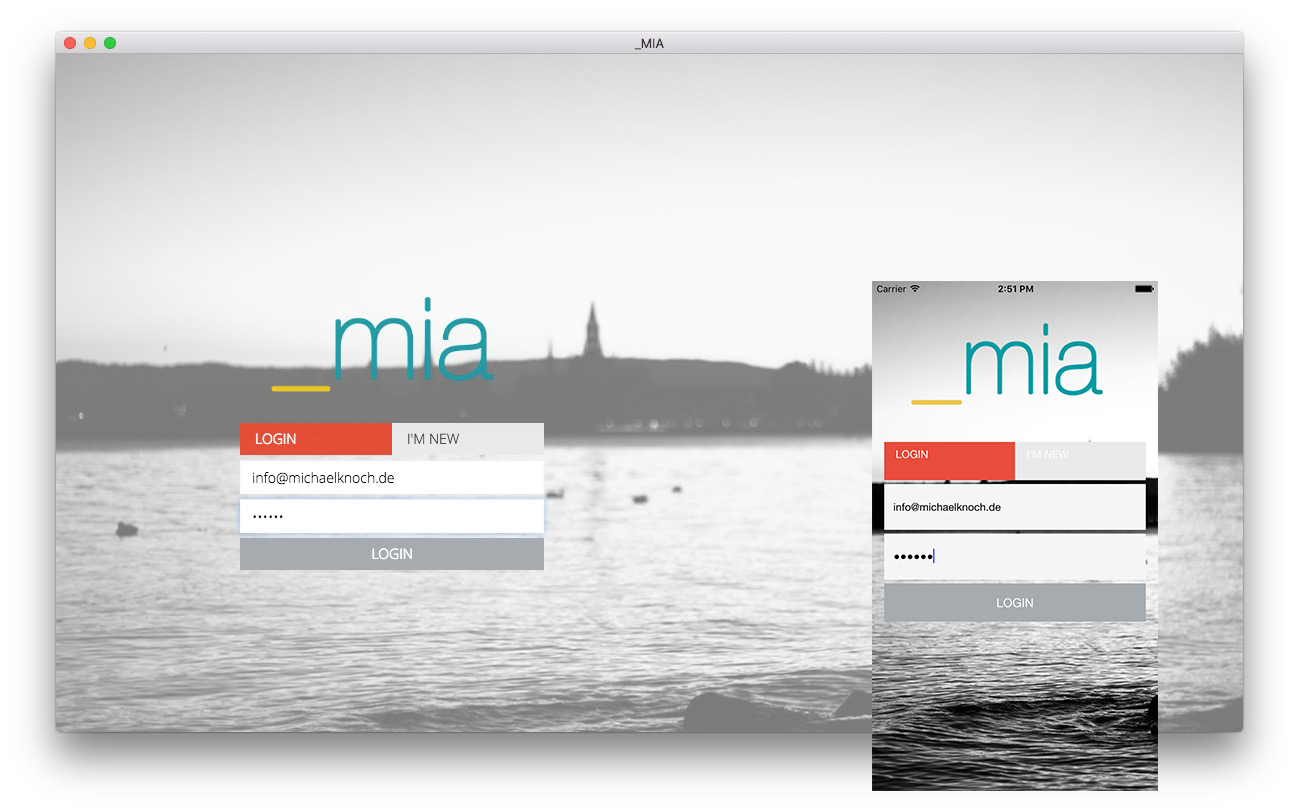
\includegraphics[width=0.9\linewidth]{appendix/app/login.png}
 \caption{Login}
\end{figure}

\begin{figure}[h!p]
 \centering
 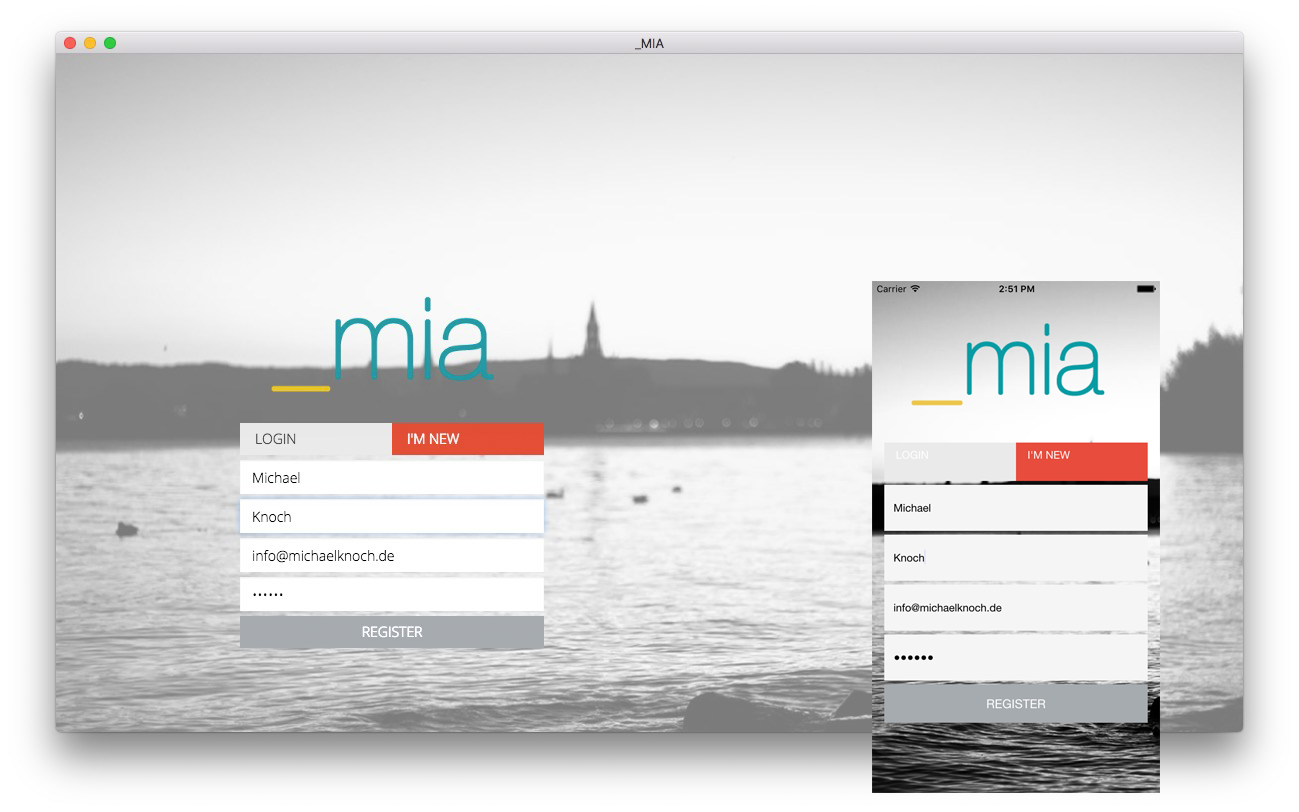
\includegraphics[width=0.9\linewidth]{appendix/app/register.png}
 \caption{Register}
\end{figure}

\begin{figure}[h!p]
 \centering
 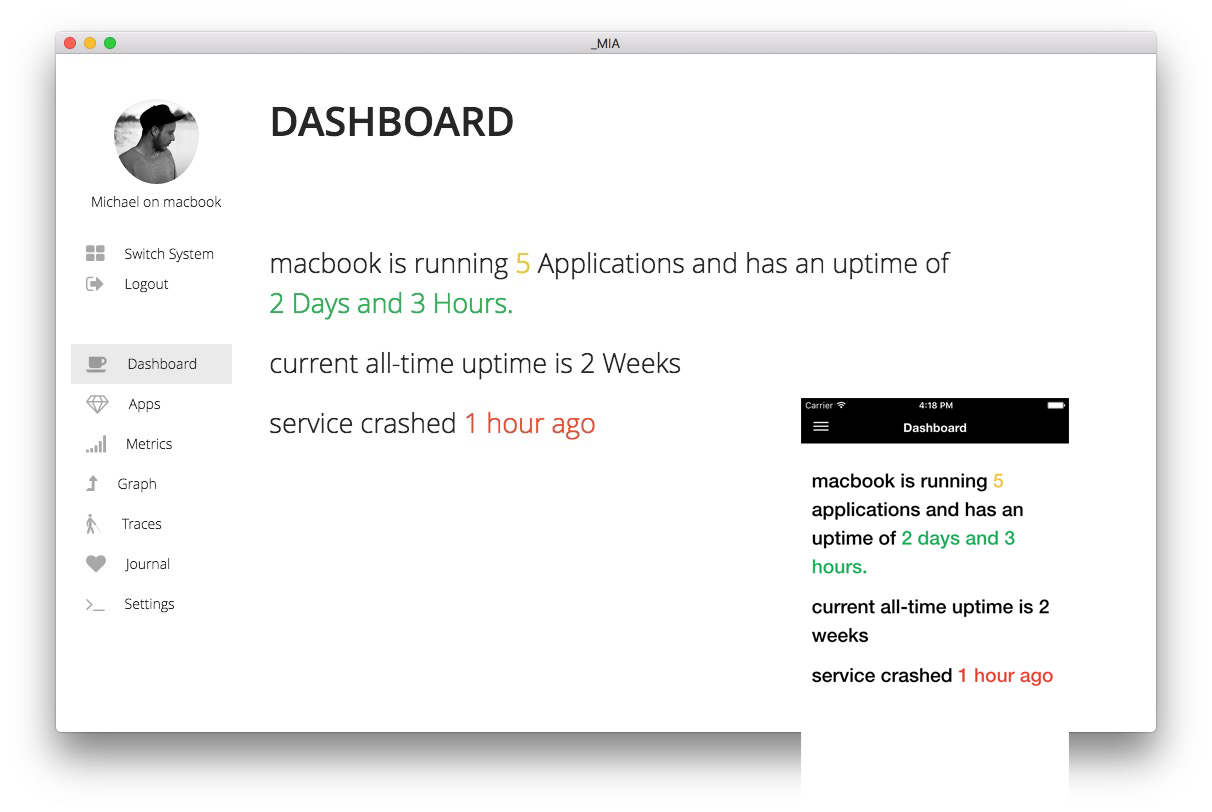
\includegraphics[width=0.9\linewidth]{appendix/app/dashboard.png}
 \caption{Dashboard}
\end{figure}

\begin{figure}[h!p]
 \centering
 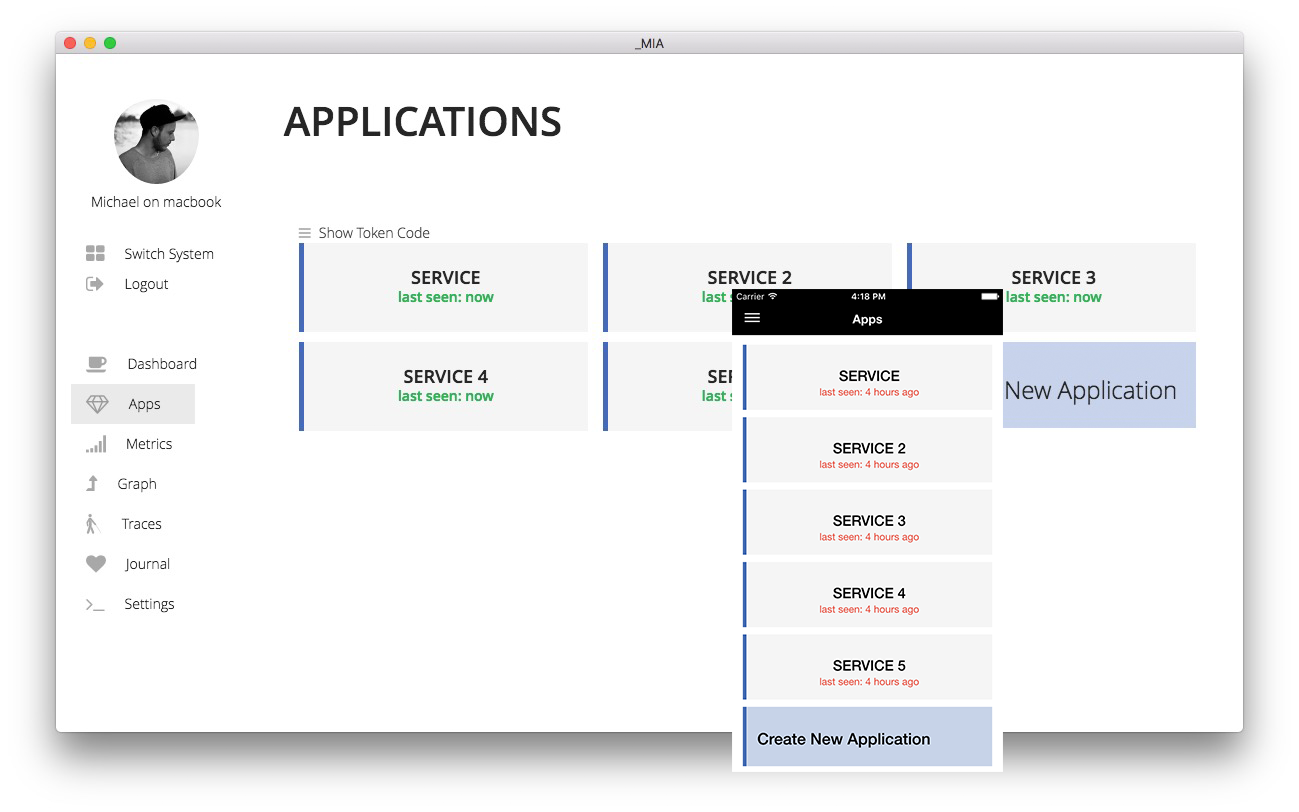
\includegraphics[width=0.9\linewidth]{appendix/app/apps.png}
 \caption{Applications}
\end{figure}

\begin{figure}[h!p]
 \centering
 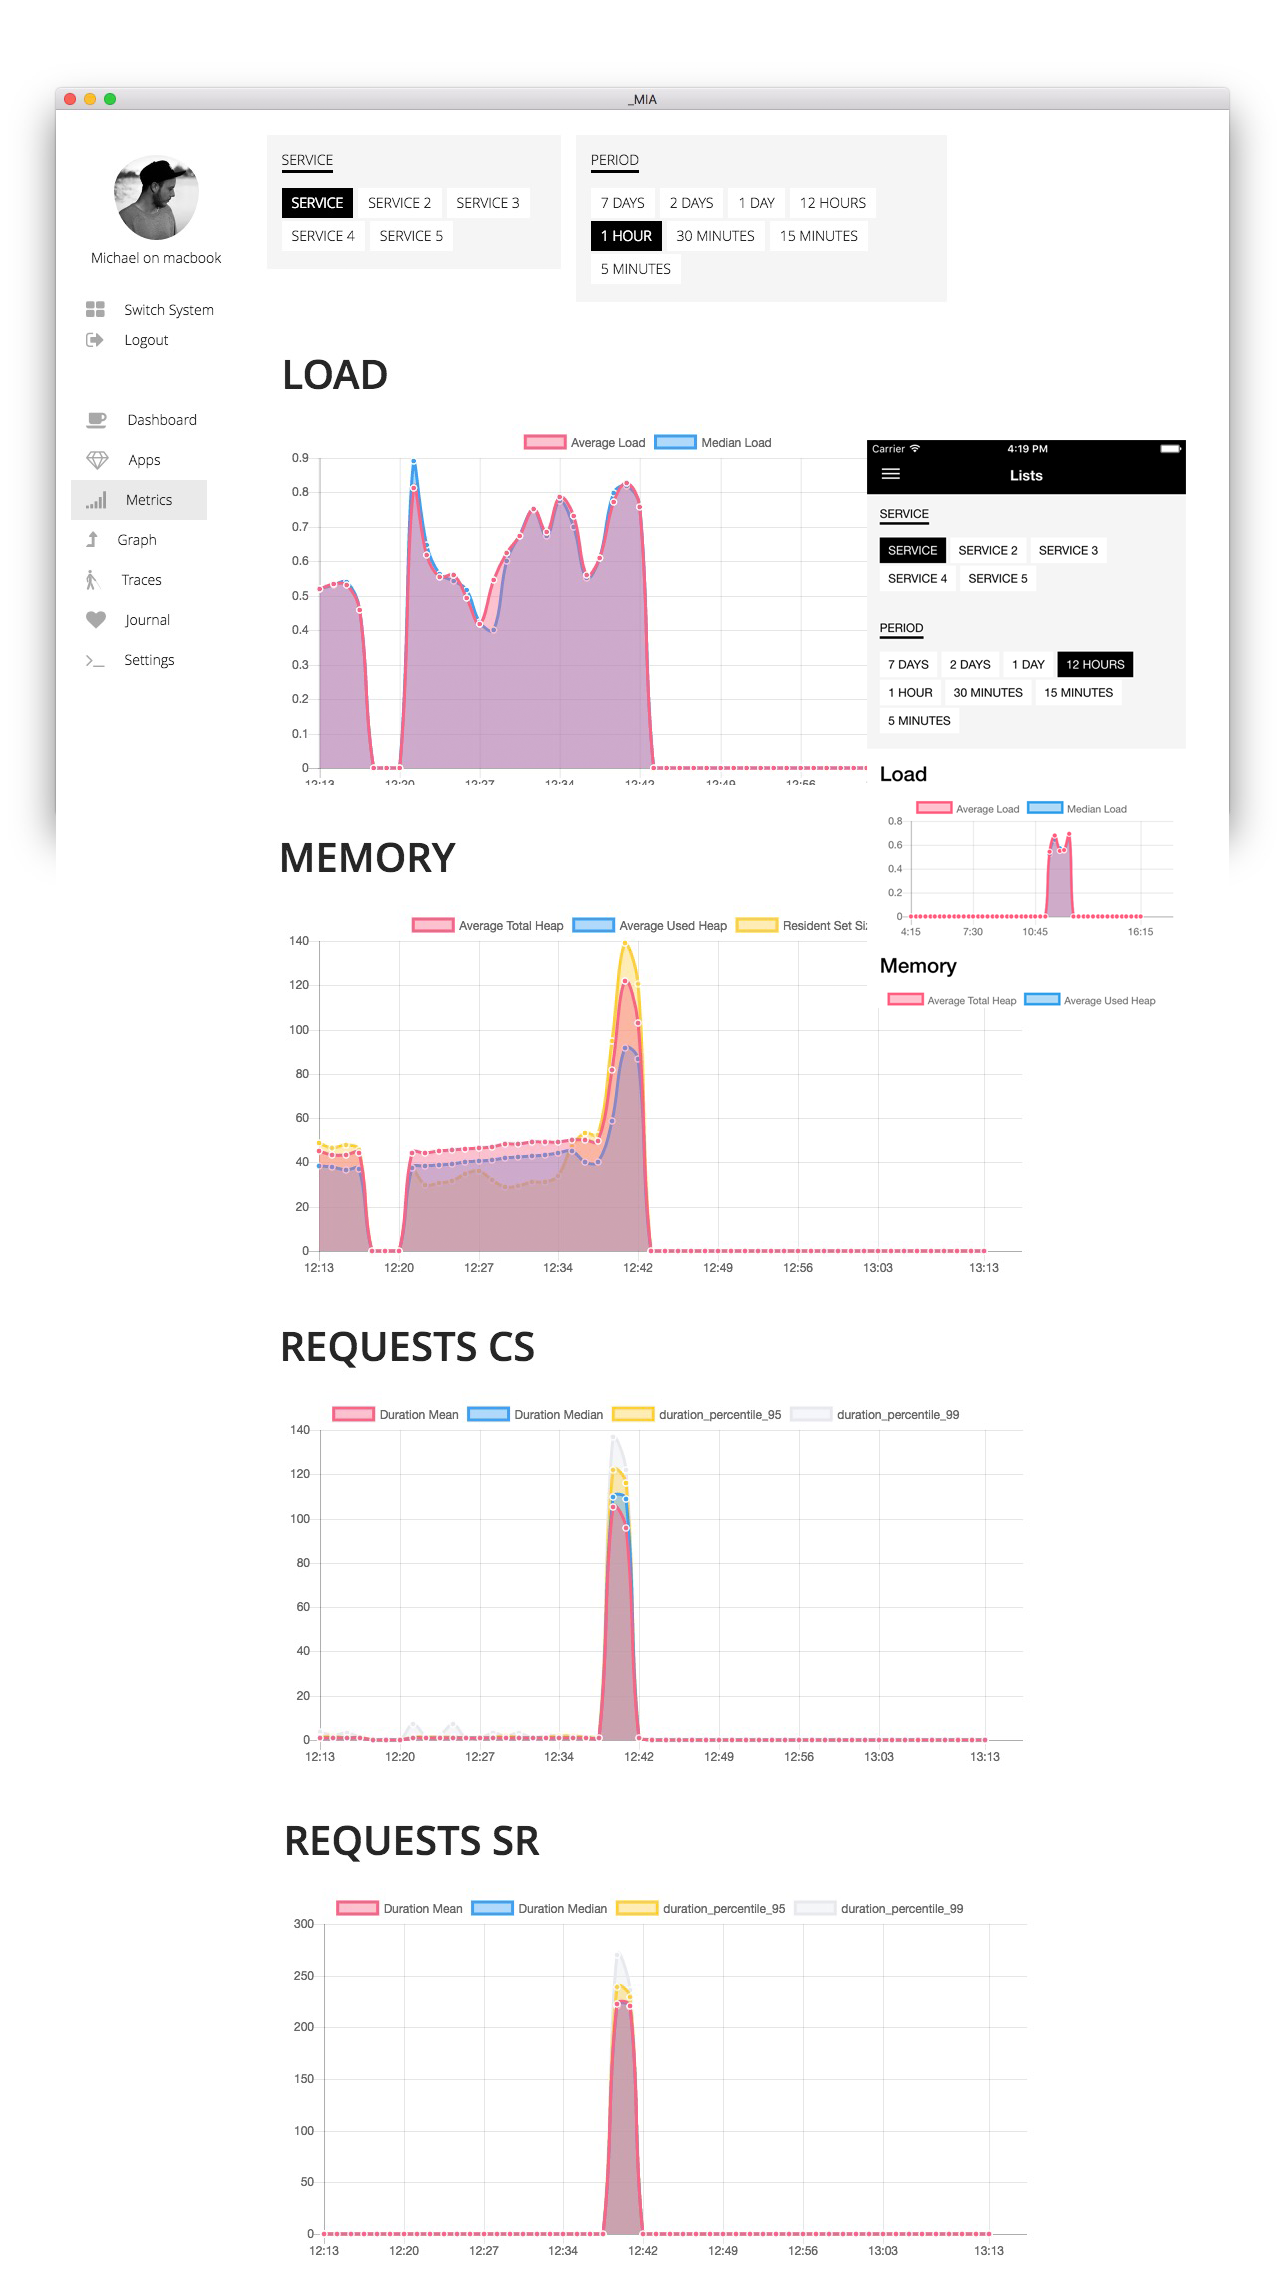
\includegraphics[width=0.9\linewidth]{appendix/app/metrics.png}
 \caption{Metrics}
\end{figure}


\begin{figure}[h!p]
 \centering
 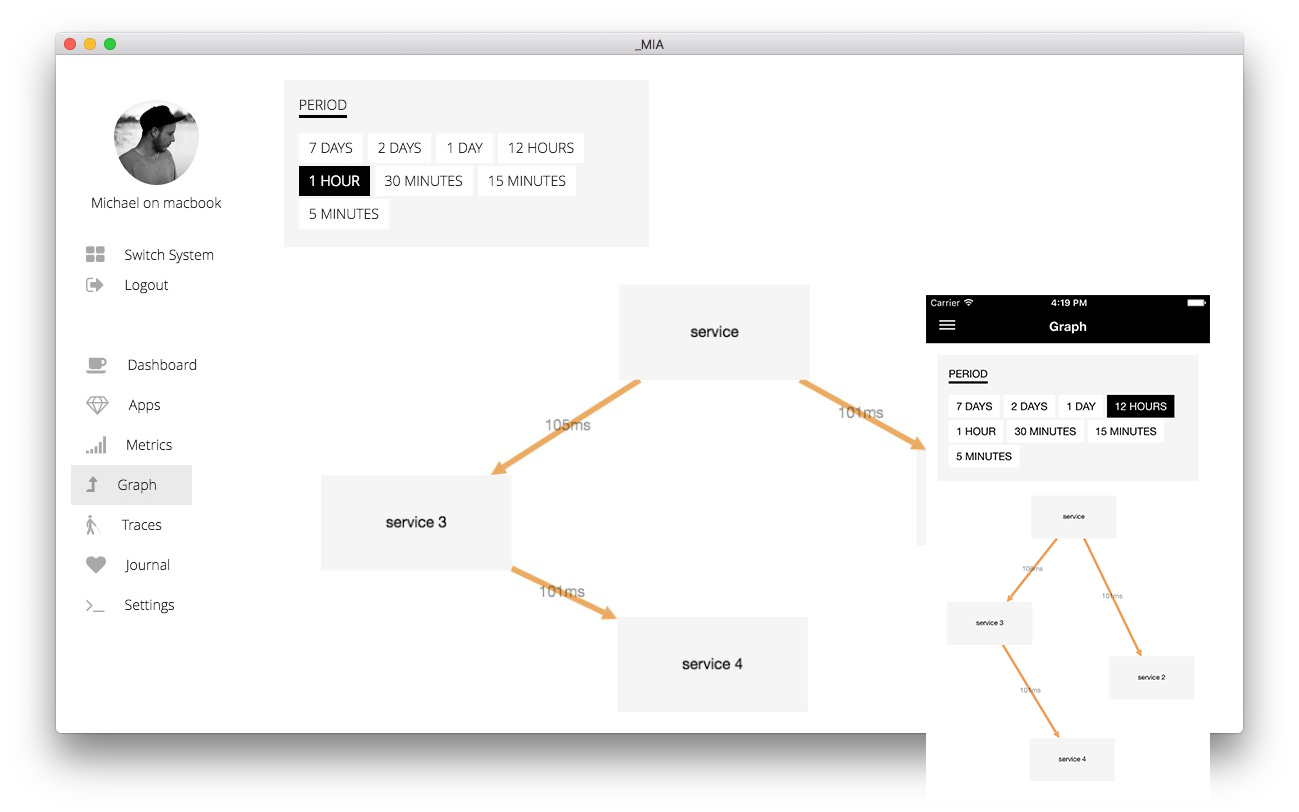
\includegraphics[width=0.9\linewidth]{appendix/app/graph.png}
 \caption{Graph}
\end{figure}

\begin{figure}[h!p]
 \centering
 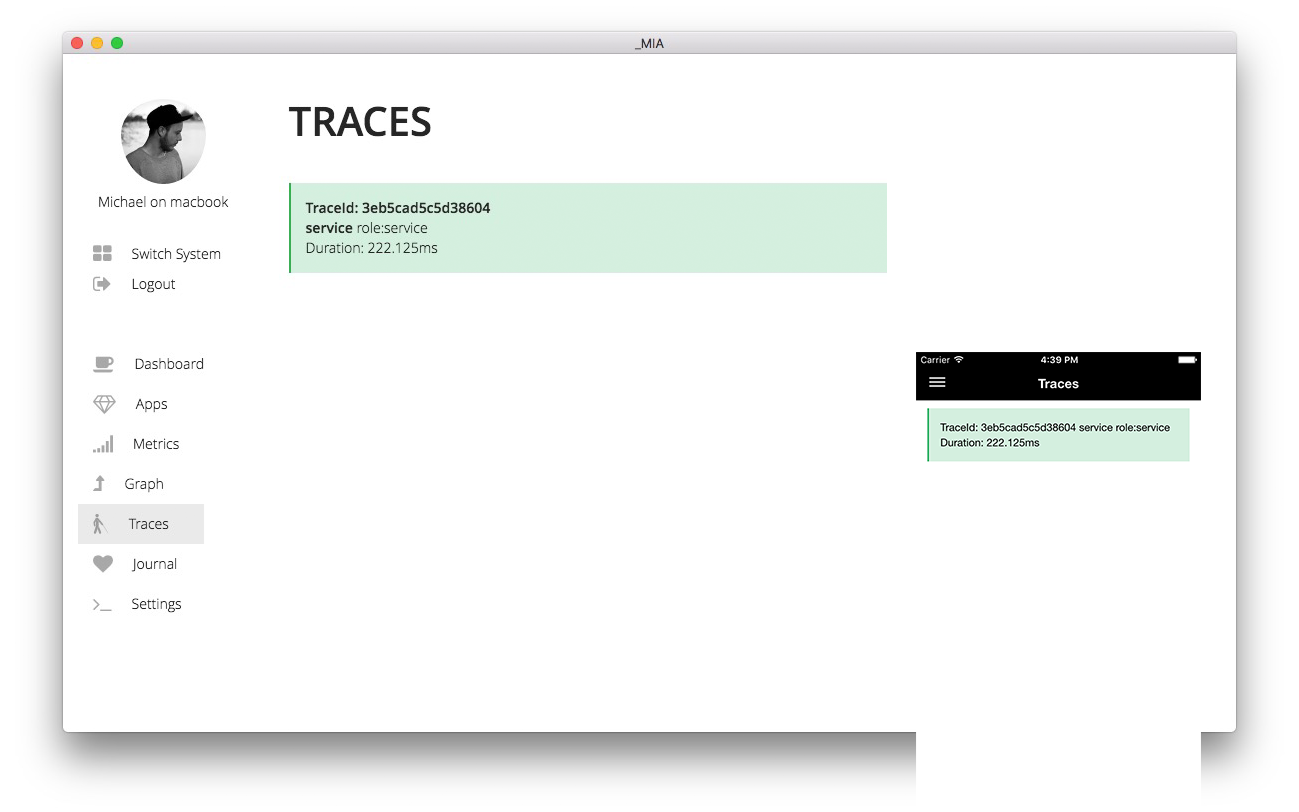
\includegraphics[width=0.9\linewidth]{appendix/app/tracelist.png}
 \caption{Tracelist}
\end{figure}

\begin{figure}[h!p]
 \centering
 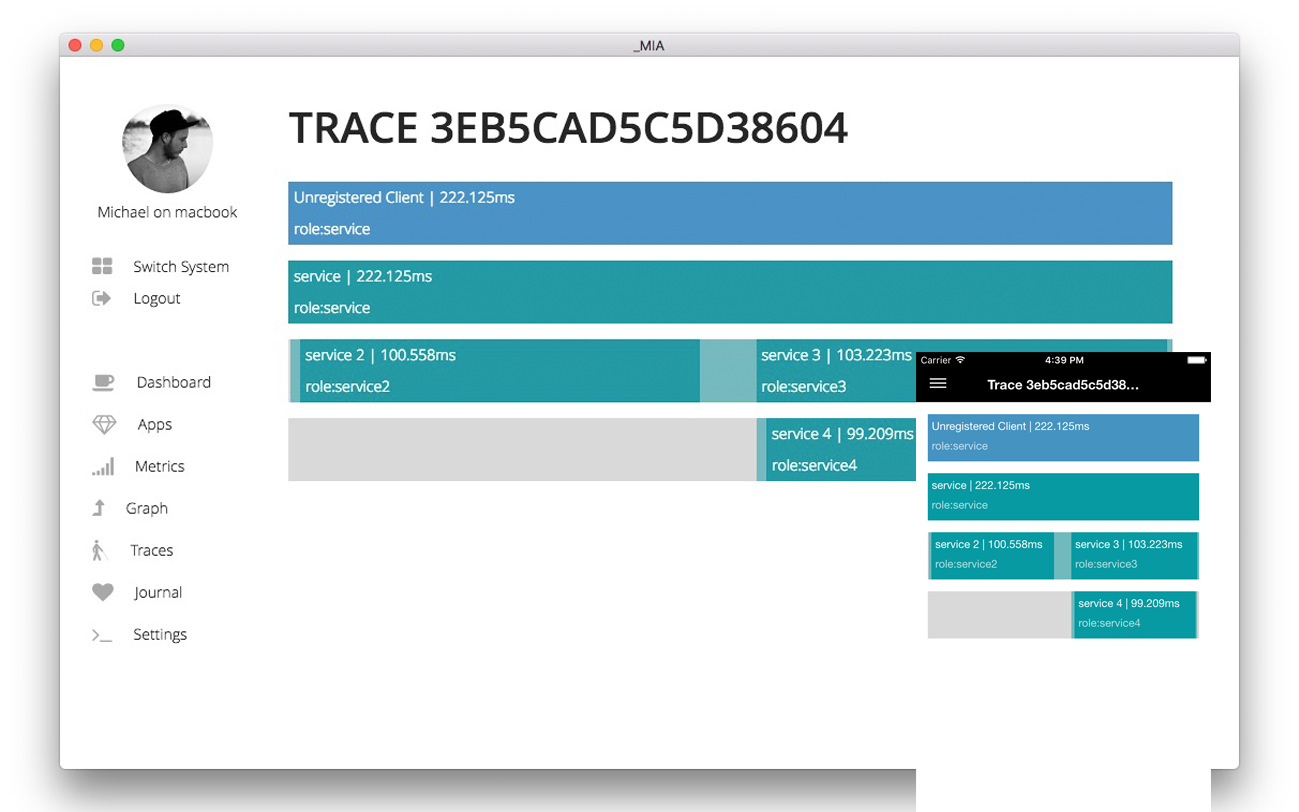
\includegraphics[width=0.9\linewidth]{appendix/app/trace-detail.png}
 \caption{Single Trace}
\end{figure}

\begin{figure}[h!p]
 \centering
 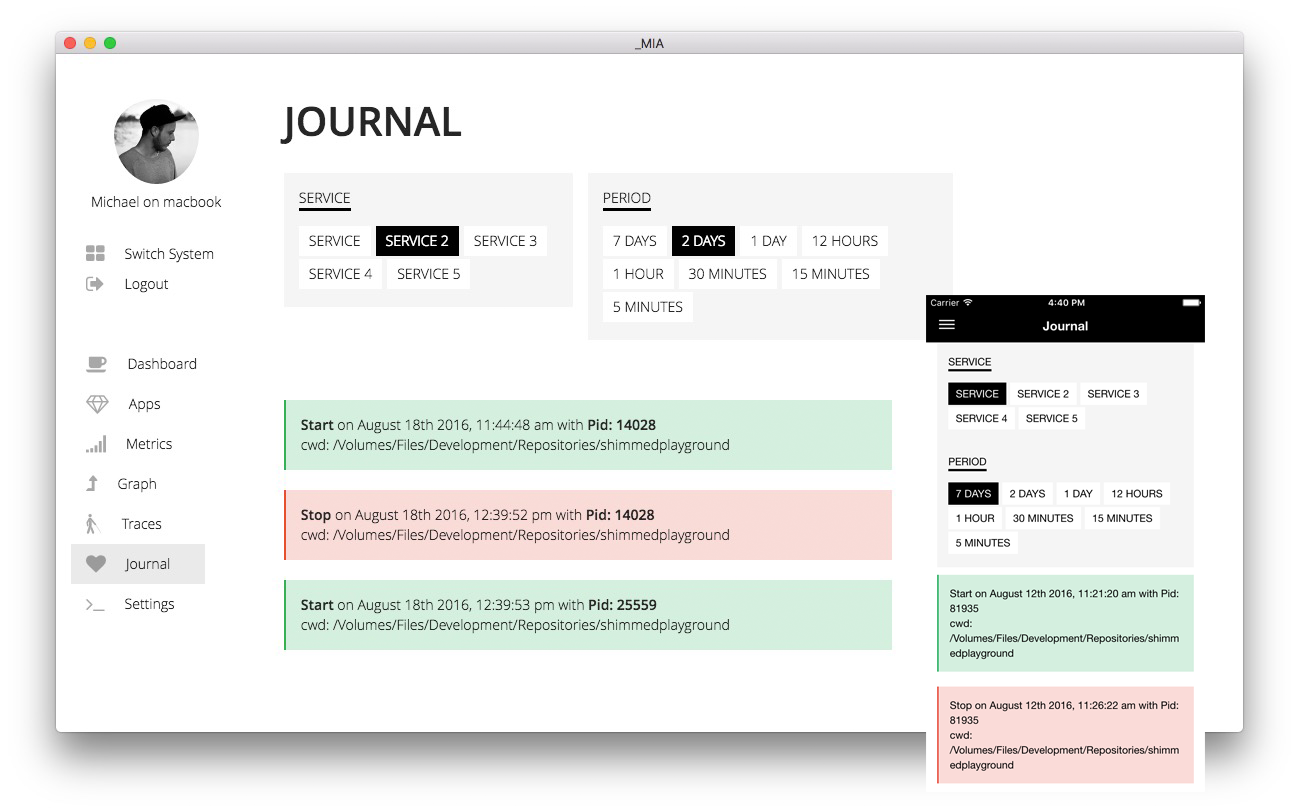
\includegraphics[width=0.9\linewidth]{appendix/app/journal.png}
 \caption{Journal}
\end{figure}

\newpage

\section{Bootstrap Timeline - Chrome Developer Tools}
\label{profiling}

\begin{figure}[h!p]
 \centering
 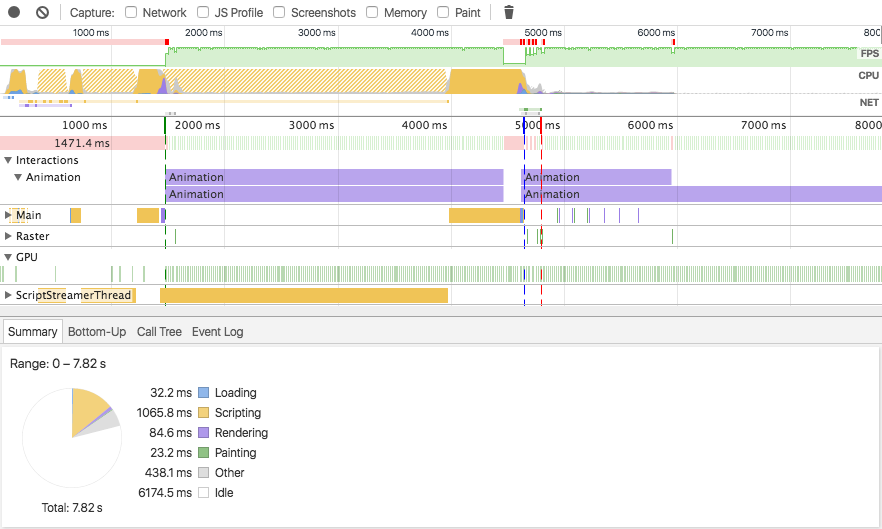
\includegraphics[width=0.9\linewidth]{appendix/profile-web.png}
 \caption{Bootstrap Timeline Web}
 \label{bootstrap-web}
\end{figure}

\begin{figure}[h!p]
 \centering
 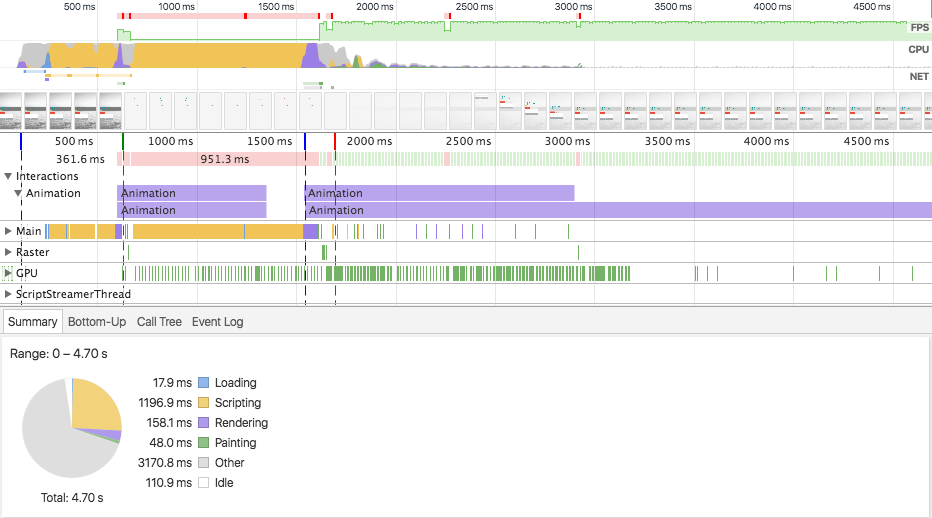
\includegraphics[width=0.9\linewidth]{appendix/profile-electron.png}
 \caption{Bootstrap Timeline Desktop}
  \label{bootstrap-desktop}
\end{figure}
